\documentclass[a4paper]{article}
\usepackage[T1]{fontenc}			% pacchetto per \chapter
\usepackage[italian]{babel}
\usepackage[italian]{isodate}  		% formato delle date in italiano
\usepackage{graphicx}				% gestione delle immagini
\usepackage{amsfonts}
\usepackage{booktabs}				% tabelle di qualità superiore
\usepackage{mathrsfs, amsmath}				% pacchetto matematica
\usepackage{mathtools}				% per sottolineare sotto le equazioni
\usepackage{stmaryrd} 				% per '\llbracket' e '\rrbracket'
\usepackage{amsthm}					% teoremi migliorati
\usepackage{enumitem}				% gestione delle liste
\usepackage{pifont}					% pacchetto con elenchi carini
\usepackage{enumitem}				% pacchetto per elenchi con lettere dell'alfabeto
\usepackage{cancel}					% per cancellare delle espressioni matematiche
\usepackage{listings}				% implementa codice di programmazione
\usepackage{mathalpha}
\usepackage{caption}


\usepackage[x11names]{xcolor}		% pacchetto colori RGB
% Link ipertestuali per l'indice
\usepackage{xcolor}
\usepackage[linkcolor=black, citecolor=blue, urlcolor=cyan]{hyperref}
\hypersetup{
	colorlinks=true
}

% Colour code style
\definecolor{codegreen}{rgb}{0,0.6,0}
\definecolor{codegray}{rgb}{0.5,0.5,0.5}
\definecolor{codepurple}{rgb}{0.58,0,0.82}
\definecolor{backcolour}{rgb}{0.95,0.95,0.92}

\lstdefinestyle{MATLAB}{
	backgroundcolor=\color{backcolour},   
	commentstyle=\color{codegreen},
	keywordstyle=\color{magenta},
	numberstyle=\tiny\color{codegray},
	stringstyle=\color{codepurple},
	basicstyle=\ttfamily\footnotesize,
	breakatwhitespace=false,         
	breaklines=true,                 
	captionpos=b,                    
	keepspaces=true,                 
	numbers=left,                    
	numbersep=5pt,                  
	showspaces=false,                
	showstringspaces=false,
	showtabs=false,                  
	tabsize=2
}
\lstset{style=MATLAB}

%\usepackage{showframe}				% visualizzazione bordi
%\usepackage{showkeys}				% visualizzazione etichetta

\newtheorem{theorem}{\textcolor{Red3}{\underline{Teorema}}}
\newtheorem{lemma}{Lemma}
\renewcommand{\qedsymbol}{QED}
\newcommand{\exec}[1]{\llbracket #1\:\rrbracket}
\newcommand{\dquotes}[1]{``#1''}
\newcommand{\longline}{\noindent\rule{\textwidth}{0.4pt}}

\begin{document}
	\author{Università degli Studi di Verona}
	\title{Soluzione - Simulazione di Elaborazione di segnali e immagini}
	\date{{\Large 29 Gennaio 2020}}
	\maketitle
	
	\section{Soluzione Esercizio}
	
	La convoluzione può essere riscritta come il prodotto tra i due segnali:
	\begin{equation*}
		y\left(t\right) = \displaystyle\int_{-\infty}^{\infty} x\left(\tau\right) \cdot h\left(t - \tau\right) \mathrm{d}\tau = \int_{-\infty}^{\infty} h\left(\tau\right) \cdot x\left(t-\tau\right) \mathrm{d}\tau
	\end{equation*}
	Assumendo che il segnale $h\left(t\right)$, che per convenzione scriveremo $h\left(f\right)$, negli estremi sia uguale a zero, si esegue una convoluzione grafica. Quindi, si evidenziano con le lettere $a,b,c$ e $d$ i vari spostamenti:
	\begin{figure}[!htp]
		\centering
		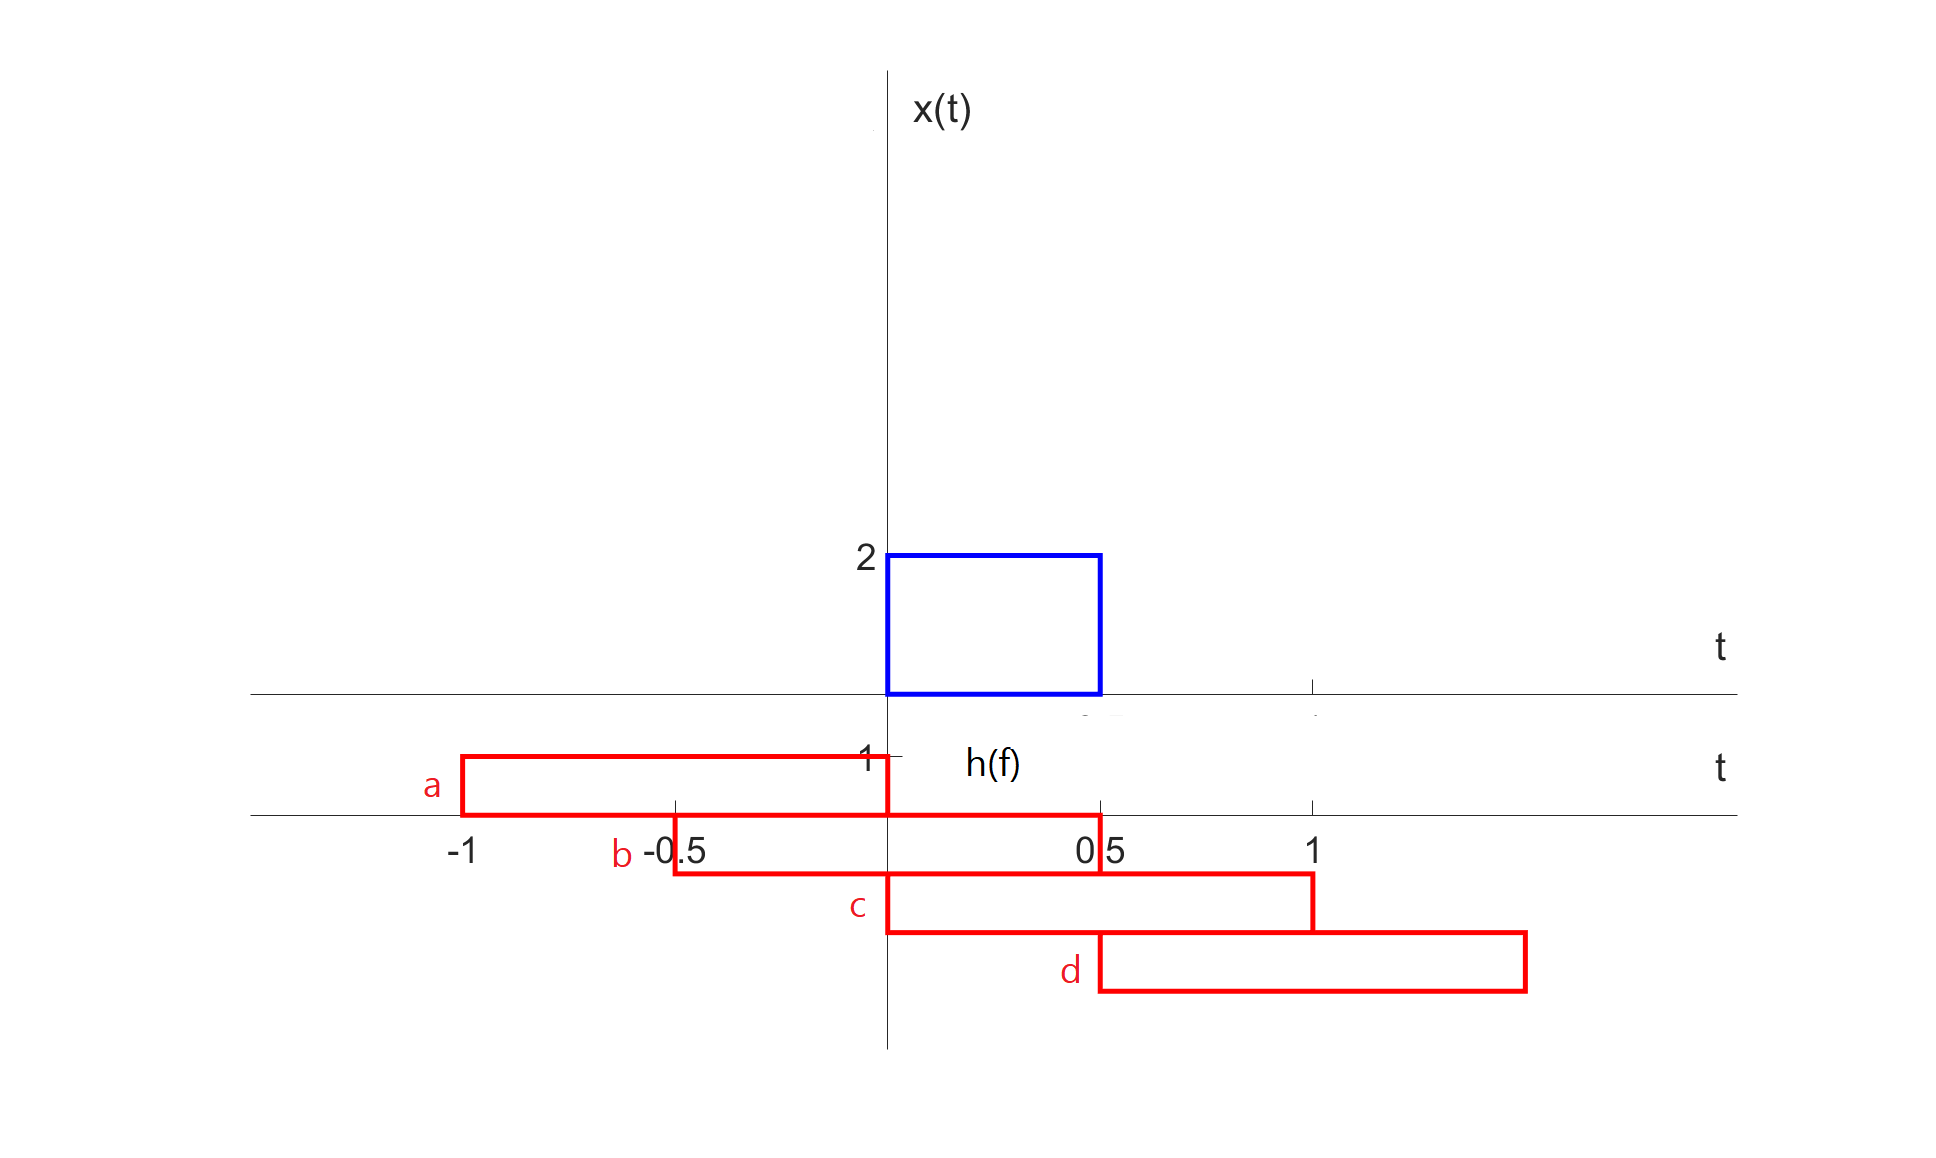
\includegraphics[width=\textwidth]{img/fig_1.png}
	\end{figure}\newpage

	\noindent
	Ad ogni spostamento del segnale $h\left(f\right)$, si costruisce graficamente l'area del segnale risultante, ovvero $y\left(t\right)$:
	\begin{figure}[!htp]
		\centering
		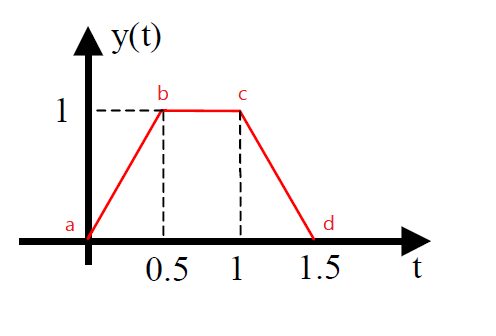
\includegraphics[width=.4\textwidth]{img/fig_2.png}
	\end{figure}

	\section{Soluzione Esercizio}
	
	Assumendo che i segnali siano rappresentati nel dominio del tempo discreto, allora la loro convoluzione corrisponde come il prodotto tra i due segnali:
	\begin{equation*}
		\begin{array}{lcl}
			y\left(t\right) & = & \displaystyle\sum_{\tau} x\left(\tau\right) \cdot h\left(t - \tau\right) \\
			& | & \\
			& = & \displaystyle\sum_{\tau} h\left(\tau\right) \cdot x\left(t - \tau\right) \\
			& | & \\
			& = & \displaystyle\sum_{\tau} h\left(\tau\right) \cdot 2\delta\left(t-0.5\right) \\
			\\
			& \downarrow & \text{Proprietà di setacciamento} \\
			\\
			& = & 2 \cdot h\left(t-0.5\right)
		\end{array}
	\end{equation*}
	Graficamente il segnale $y\left(t\right)$ risulta uguale a zero fino al valore $0.5$, ovvero finché il segnale $h\left(t\right)$ interseca il segnale $x\left(t\right)$. Dopodiché, rimane di ampiezza pari a $2$ fino al valore $1.5$, ovvero l'ultima intersezione registrata durante la convoluzione (per la convoluzione grafica si guardi la soluzione precedente):
	\begin{figure}[!htp]
		\centering
		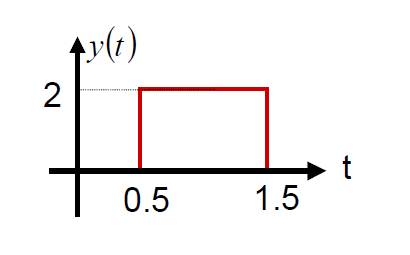
\includegraphics[width=.4\textwidth]{img/fig_3.png}
	\end{figure}

	\noindent
	\textbf{Nota}: il valore $x\left(t-\tau\right)$ è pari a $2\delta\left(t-0.5\right)$ poiché è stato fornito dal testo dell'esercizio.\newpage
	
	\section{Soluzione Esercizio}
	
	La soluzione dell'esercizio prevede 3 casi per 3 valori di campionamento diverso. Nel primo caso (\emph{a}) si determina anche il risultato (output) grafico del campionamento nel dominio del tempo continuo e nel dominio delle frequenze.
	
	\subsection*{\textcolor{Green4}{\underline{Caso \emph{a}}}}
	
	Il campionamento è ogni $15$ Hz, quindi il grafico è:
	\begin{figure}[!htp]
		\centering
		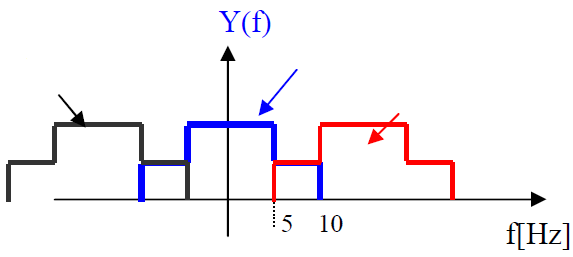
\includegraphics[width=.4\textwidth]{img/fig_4.png}
	\end{figure}

	\noindent
	L'ampiezza del segnale diventa $30$ ($2 \times 15$). Anche senza il teorema di Nyquist\footnote{\href{https://it.wikipedia.org/wiki/Teorema_del_campionamento_di_Nyquist-Shannon}{Teorema di Nyquist}} è possibile notare l'aliasing.\newline
	
	\noindent
	Il risultato post campionamento è un segnale costante di ampiezza $30$ (si ricorda che il campionamento è la moltiplicazione del segnale per un treno di impulsi):
	\begin{figure}[!htp]
		\centering
		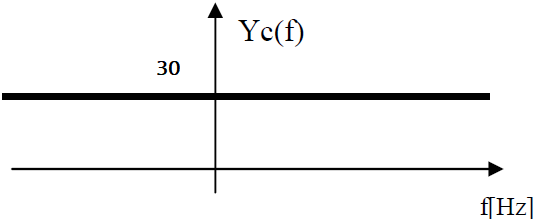
\includegraphics[width=.4\textwidth]{img/fig_5.png}
	\end{figure}

	\noindent
	Nel dominio delle frequenze, il segnale è un impulso centrato in $0$ con ampiezza pari a $30$:
	\begin{figure}[!htp]
		\centering
		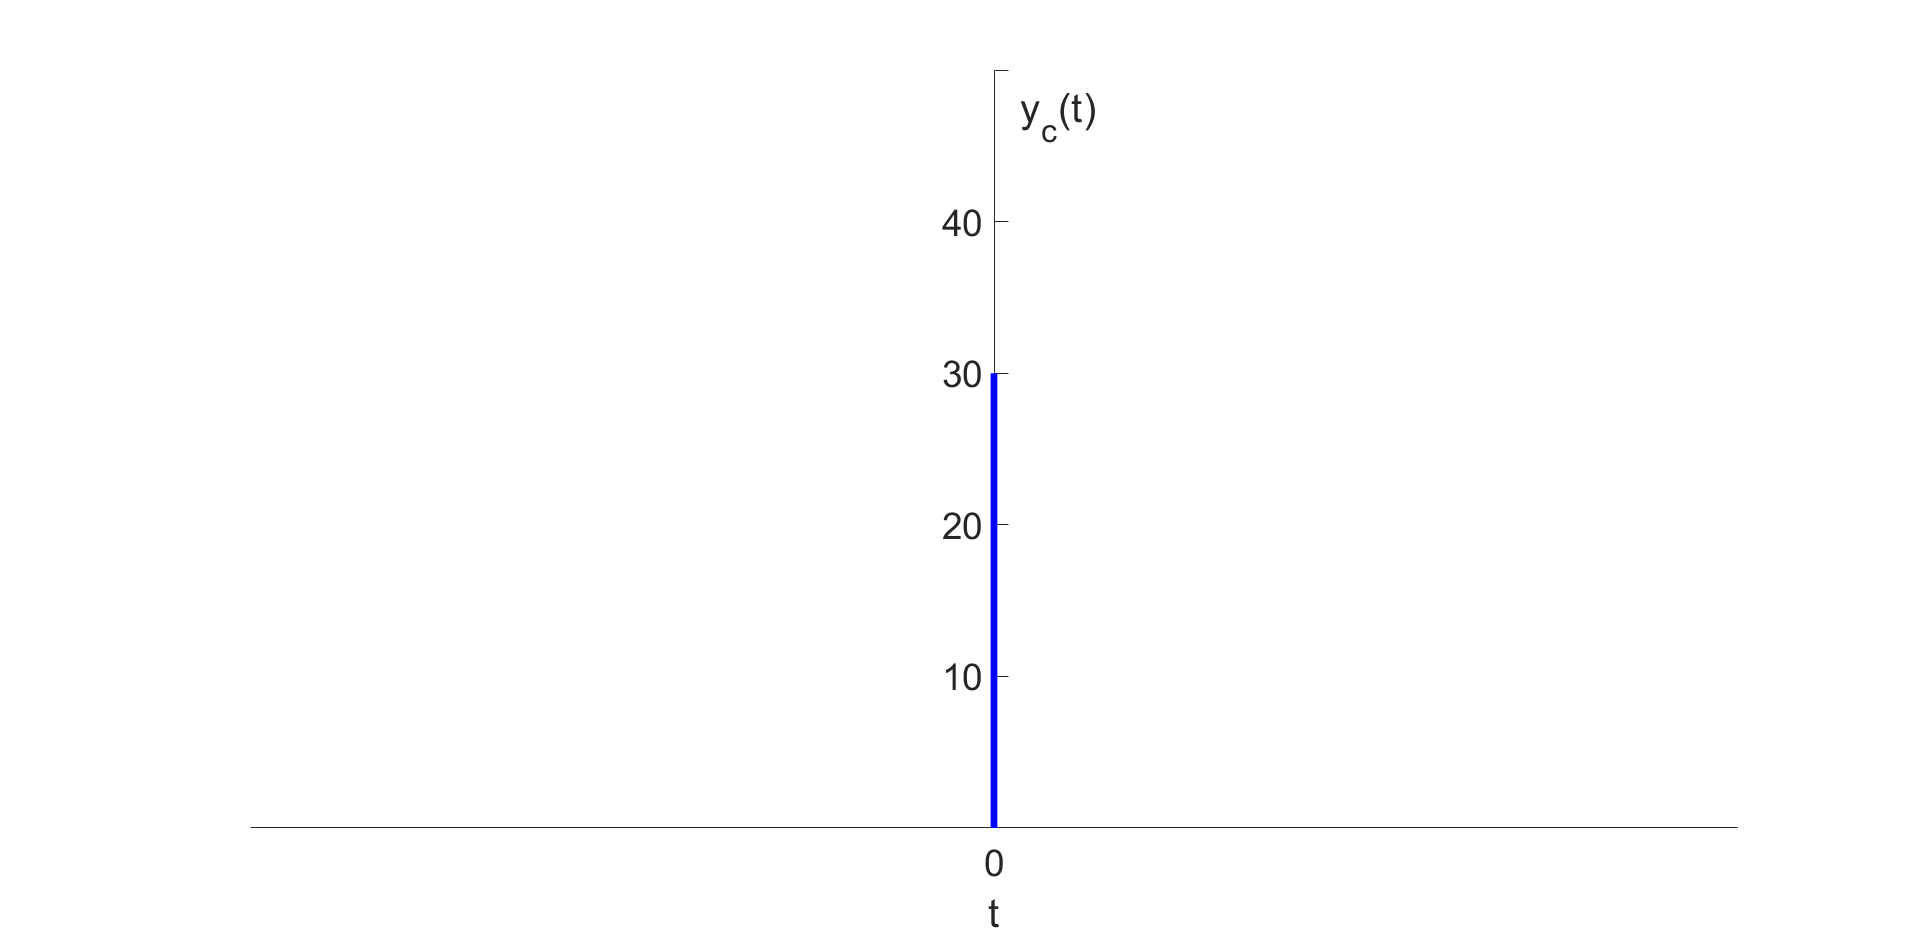
\includegraphics[width=\textwidth]{img/fig_6.png}
		\caption*{$y_{c}\left(t\right) = 30\delta\left(t\right)$}
	\end{figure}
	
	\subsection*{\textcolor{Green4}{\underline{Caso \emph{b}}}}
	
	Il campionamento è ogni $17.5$ Hz, quindi il grafico è:
	\begin{figure}[!htp]
		\centering
		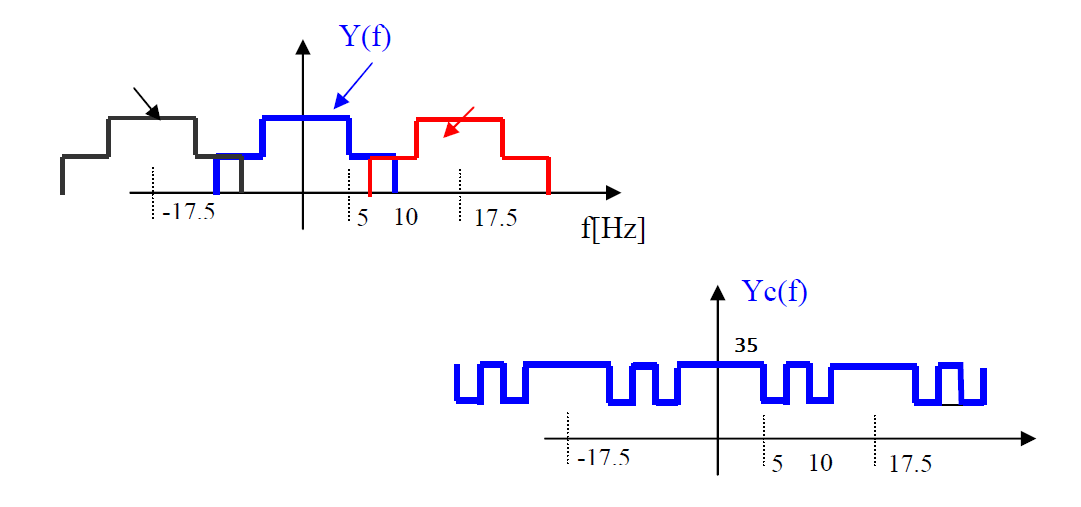
\includegraphics[width=\textwidth]{img/fig_7.png}
	\end{figure}
	
	\noindent
	L'ampiezza del segnale diventa $35$ ($2 \times 17.5$). Si manifesta aliasing.
	
	\subsection*{\textcolor{Green4}{\underline{Caso \emph{c}}}}
	
	Il campionamento è ogni $22$ Hz, quindi il grafico è:
	\begin{figure}[!htp]
		\centering
		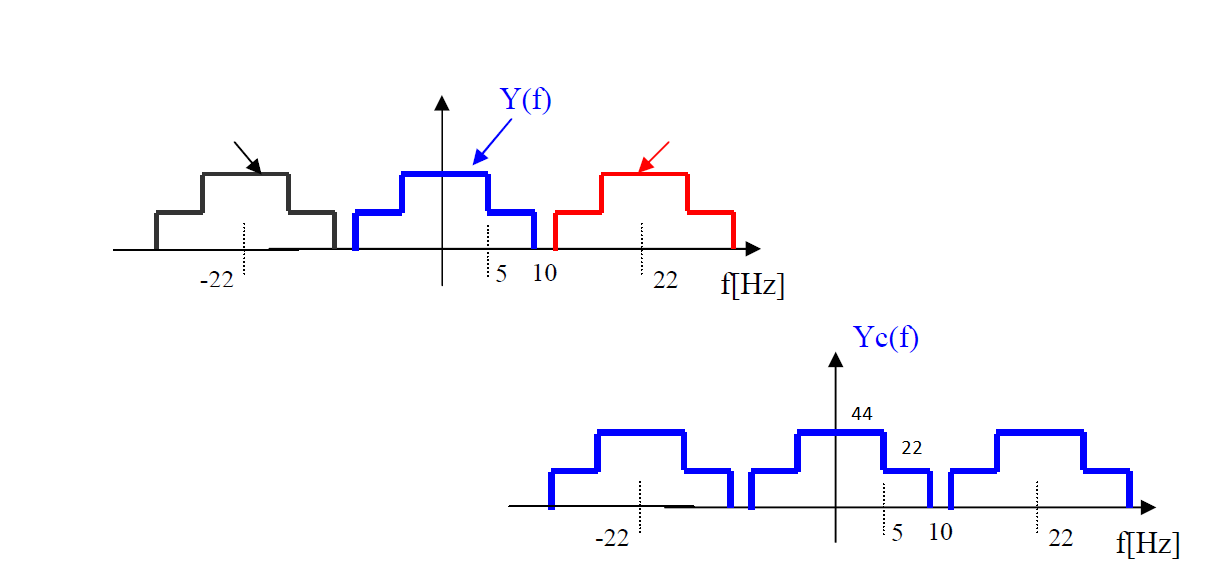
\includegraphics[width=\textwidth]{img/fig_8.png}
	\end{figure}
	
	\noindent
	L'ampiezza del segnale diventa $44$ ($2 \times 17.5$). L'aliasing non si presenta.\newpage
	
	\section{Soluzione Esercizio}
	
	Si applica il filtro di ricostruzione ideale con una frequenza che dipende a quanto è stato campionato ogni segnale.
	
	\subsection*{\textcolor{Green4}{\underline{Caso \emph{a}}}}
	
	La frequenza del campionamento è stata con una frequenza di $15$ Hz. Quindi, la frequenza di taglio del filtro di ricostruzione ideale è $7.5$ Hz $\left(15 \div 2\right)$.
	\begin{figure}[!htp]
		\centering
		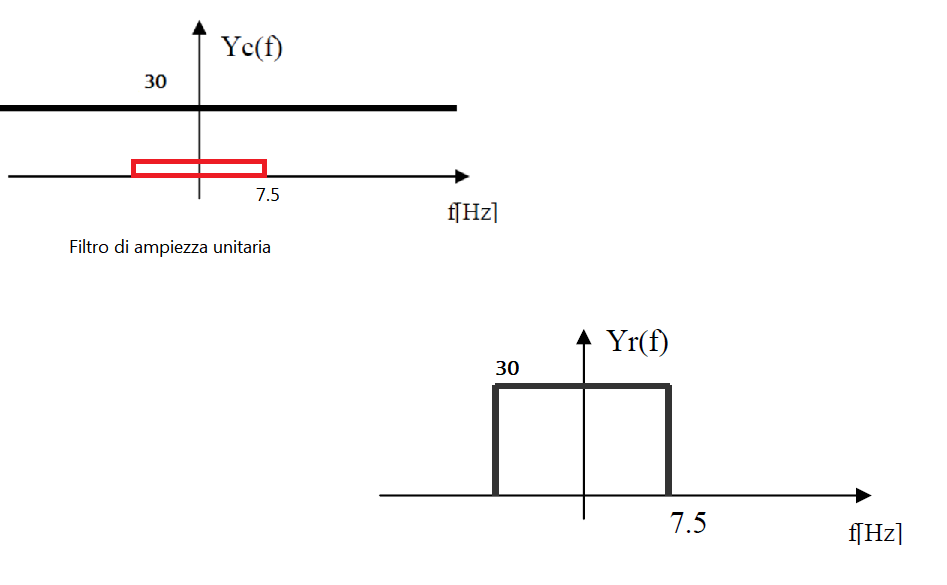
\includegraphics[width=\textwidth]{img/fig_9.png}
		\caption*{A sinistra in alto, la rappresentazione del segnale insieme al filtro e a destra in basso, la ricostruzione ideale che non corrisponde al segnale originario.}
	\end{figure}
	
	\noindent
	Il filtro, da definizione, taglia tutte le frequenze e si ottiene una box di base $15$ e altezza $30$. Dato che il segnale manifestava aliasing, il segnale \underline{non} può essere ricostruito.\newpage
	
	\subsection*{\textcolor{Green4}{\underline{Caso \emph{b}}}}
	
	La frequenza del campionamento è stata con una frequenza di $17.5$ Hz. Quindi, la frequenza di taglio del filtro di ricostruzione ideale è $8.75$ Hz $\left(17.5 \div 2\right)$.
	\begin{figure}[!htp]
		\centering
		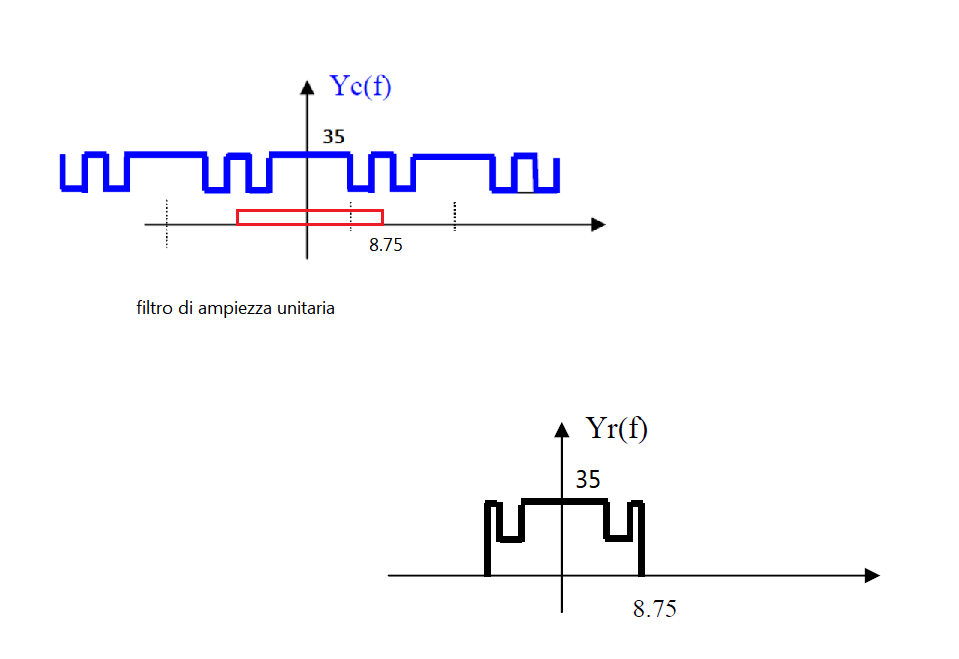
\includegraphics[width=\textwidth]{img/fig_10.png}
		\caption*{A sinistra in alto, la rappresentazione del segnale insieme al filtro e a destra in basso, la ricostruzione ideale che non corrisponde al segnale originario.}
	\end{figure}
	
	\noindent
	Il filtro, da definizione, taglia tutte le frequenze e si ottiene una box di base $17.5$ e altezza $35$. Dato che il segnale manifestava aliasing, il segnale \underline{non} può essere ricostruito.\newpage
	
	\subsection*{\textcolor{Green4}{\underline{Caso \emph{c}}}}
	
	La frequenza del campionamento è stata con una frequenza di $22$ Hz. Quindi, la frequenza di taglio del filtro di ricostruzione ideale è $11$ Hz $\left(22 \div 2\right)$.
	\begin{figure}[!htp]
		\centering
		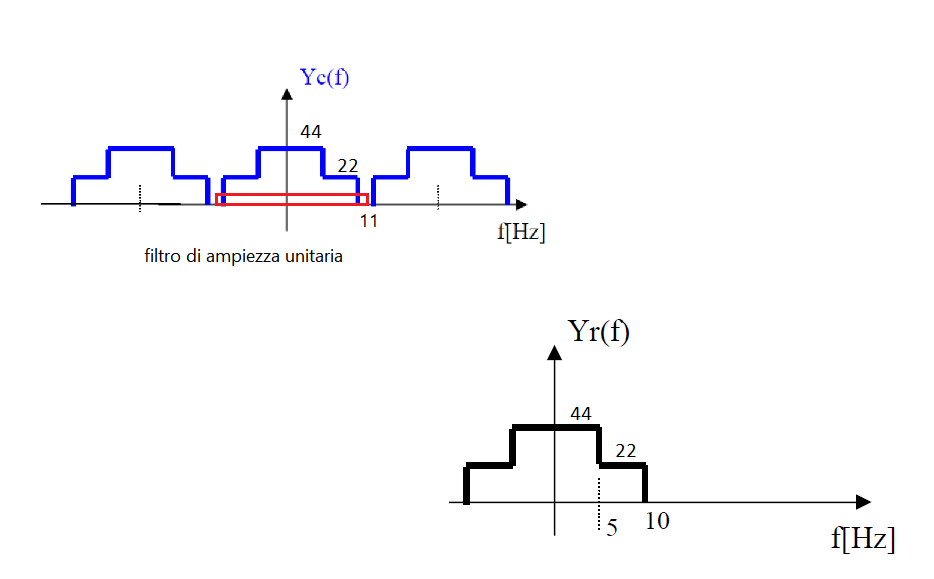
\includegraphics[width=\textwidth]{img/fig_11.png}
		\caption*{A sinistra in alto, la rappresentazione del segnale insieme al filtro e a destra in basso, la ricostruzione ideale che corrisponde al segnale originario.}
	\end{figure}
	
	\noindent
	Il filtro, da definizione, taglia tutte le frequenze e si ottiene una box di base $20$ e altezza $44$. Dato che il segnale \underline{non} manifestava aliasing, \textbf{è stato ricostruito con successo}.
\end{document}